\subsection{Squares over Unordered Alphabets}

\begin{frame}
    \centering
    {\Large Optimal Square Detection  Over General Alphabets}
  
    \bigskip
    {\large SODA'23}\\
    \bigskip
    
\includegraphics{pictures/mindmap/squares.png}
  
    \bigskip
    Jonas Ellert, Paweł Gawrychowski
\end{frame}


\begin{frame}{The use of Lempel-Ziv factorization to detect squares}
    \begin{center}
        \begin{tikzpicture}[scale=0.8, every node/.style={transform shape}]
        \tikzset{barcolor/.style={black, densely dotted}}
        \tikzset{fcolor/.style={black}}
        
        \setcounter{symbid}{0}
        \foreach[count=\factorid from 1, evaluate=\factorid as \prevfid using int(\factorid-1)] \factorset in {%
        {a},
        {b},%
        {c},
        {b,a},
        {b,a,a},
        {b,c,b,a,c},%
        {b,a,b,a,a,b,c,z},%
        {z,b},
        {a,b,a}%
        }
        {
    
            \only{
            \ifnum\factorid=7
                \tikzset{barcolor/.style={black, densely dotted}}
                \tikzset{fcolor/.style={black, font=\boldmath}}	
            \else
                \beamermathcolor{black!30!white}
                \tikzset{barcolor/.style={black!20!white, densely dotted}}
                \tikzset{fcolor/.style={barcolor}}
            \fi}
    
            \path (\thesymbid\lzspacing+0.5\lzspacing, -0.5em) node (leftbar) {};
            \foreach \tsymb in \factorset {
                \addtocounter{symbid}{1}
                \node[inner sep=0] (\thesymbid) at (\thesymbid\lzspacing,0) {\smash{\texttt{\tsymb}\vphantom{$\strut$}}$\vphantom{m}$};
                %\node at (\thesymbid\lzspacing,1) {$\scriptstyle\thesymbid$};
            }
            \path (\thesymbid\lzspacing+0.5\lzspacing, -0.5em) node (rightbar) {};
            \path (leftbar) to node[midway] (centerbar) {} (rightbar);
            %\node[above of=centerbar, fcolor] (flab\factorid) {$f_{\factorid}$};
            \node[above=.75em of centerbar |- \thesymbid.north, fcolor] (flab\factorid) {$f_{\factorid}$};
    
            \ifodd\factorid\else
                \draw[thick, barcolor] (leftbar.center) to ++(0,1);
                \draw[thick, barcolor] (rightbar.center) to ++(0,1);
            \fi
        }
    
        \tikzset{hlbox/.style={draw, ultra thick, inner xsep=2.5pt}}
    
      
        
        \foreach[count=\i from 14, evaluate=\i as \j using int(\i-10)] \x in {b,a,b,a,a,b,c} {
        \node[below=1em of \i, inner sep=0] (low\i) {\smash{\texttt{\x}\vphantom{$\strut$}}$\vphantom{m}$};
        \node[below=1em of \j, inner sep=0] (low\j) {\smash{\texttt{\x}\vphantom{$\strut$}}$\vphantom{m}$};
        }
    
        \only{
            \node[hlbox, fit=(low14)(low20), myblue] (ma) {};
    
            \node[below=0 of ma] (malab) {\bblue{already seen}};
    
        }
        \node[hlbox, fit=(low4)(low10), myblue] (fi) {};
    
        
        \node[below=1em of 21, inner sep=0] (low21) {\smash{\texttt{z}\vphantom{$\strut$}}$\vphantom{m}$};
        \node[below=1em of 11, inner sep=0] (low11) {\smash{\texttt{b}\vphantom{$\strut$}}$\vphantom{m}$};
        \node[hlbox, fit=(low21), mygreen] {};
        \node[hlbox, fit=(low11), mygreen] {};
    
        \draw node[left=0 of 1] {$w = \strut$};
        \end{tikzpicture}
    \end{center}
    \pause
    We process $w$ \ntheme{left to right}, square testing, we can note that:\pause
    \begin{itemize}
        \item<3-> We don't have to look for a square fully included in $f_i[..-1]$.
        \item<6-> If the previous occurrence of $f_i[..-1]$ overlaps with itself, then it implies a square.
        \item<8-> The right arm of square can overlap at most two phrases.
        \item<12-> For $x$ and $y$ square-free string we can detect squares in $xy$ with their right arm in $y$ contained in $\Oh(|y|)$ time.
    \end{itemize}


    \begin{center}
    \begin{tikzpicture}[scale=0.9, every node/.style={transform shape}]
        \beamermathcolor{black}
        \onslide<1->{
        
        \node (0) {$\qquad\quad w = {}$};
        \foreach[evaluate=\i as \iminus using int(\i-1)] \i in {1,...,30} {
            \node[right=0 of \iminus, minimum width=1.05em] (\i) {\vphantom{a}};
            \node[below=-0.25em of \i, minimum width=1.05em] (d\i) {\vphantom{a}};
        }

        % Arrow occurs before
        \only<5|handout:0>{
            \node[fit=(6)(7), fill=mygreen!40!white, inner sep=0pt] (flarm) {};
            \node[fit=(8)(9), fill=mygreen!40!white, inner sep=0pt] (frarm) {};
            \node at (flarm.center) {$\alpha$};
            \node at (frarm.center) {$\alpha$};
            \node[fit=(6)(7), thick, draw=black, inner sep=0pt] (flarm) {};
            \node[fit=(8)(9), thick, draw=black, inner sep=0pt] (frarm) {};
            \draw[-latex] (larm) to[out=-90, in=-90] (flarm);
        }

        % small square
        \only<4-5|handout:0>{
            \node[fit=(14)(15), fill=mygreen!40!white, inner sep=0pt] (olarm) {};
            \node[fit=(16)(17), fill=mygreen!40!white, inner sep=0pt] (orarm) {};
            \node at (olarm.center) {$\alpha$};
            \node at (orarm.center) {$\alpha$};
            \node[fit=(14)(15), thick, draw=black, inner sep=0pt] (olarm) {};
            \node[fit=(16)(17), thick, draw=black, inner sep=0pt] (orarm) {};
        }

    
        
        \node[fit=(1)(30), draw=black, inner sep=0pt] {};
        
        \tikzset{barcolor/.style={densely dotted}}
        \tikzset{fcolor/.style={}}
        
        \onslide<1->{
        
        \foreach[%
        evaluate=\len as \lensum using int(\prevlensum+\len), %
        evaluate=\prevlensum as \starti using int(\prevlensum+1),
        remember=\lensum as \prevlensum initially 0,
        count=\j from 1] %
        \len in {1,2,4,6,5,5,7} {
        
            \node[fit=(\starti)(\lensum), inner sep=0pt] (fact\j) {};
        
            \only<6->{
            \ifnum\j=6
                \tikzset{barcolor/.style={black, densely dotted}}
                \tikzset{fcolor/.style={font=\boldmath}}
            \else
                \beamermathcolor{black!30!white}
                \tikzset{barcolor/.style={black!30!white, densely dotted}}
                \tikzset{fcolor/.style={black!30!white}}
            \fi}
            
            \node[above=0.25em of fact\j, fcolor] (flab\j) {$f_{\j}$};
            
            \ifodd\j\else\ifnum\j=6
                \draw[thick, barcolor] (fact\j.south west) ++(0,-.002) to ++(0,1.002);
                \draw[thick, barcolor] (fact\j.south east) ++(0,-.002) to ++(0,1.002);
            \else
                \draw[thick, barcolor] (fact\j.south west) ++(0,-.002) to ++(0,1.002);
                \draw[thick, barcolor] (fact\j.south east) ++(0,-.002) to ++(0,1.002);
            \fi\fi
        }

        % OVERLAP WITH ITSELF
        \onslide<7|handout:0>{
            \node[fit=(17)(18), fill=mygreen!40!white, inner sep=0pt] (larm) {};
            \node[fit=(19)(20), fill=mygreen!40!white, inner sep=0pt] (rarm) {};
            \node at (larm.center) {$\alpha$};
            \node at (rarm.center) {$\alpha$};
            \node[fit=(17)(18), thick, draw=black, inner sep=0pt] (larm) {};
            \node[fit=(19)(20), thick, draw=black, inner sep=0pt] (rarm) {};
        }  
            
        \onslide<6-7|handout:0>{
        \node[fit=(d17)(d21), thick, fill=myblue!50!white, draw=black, inner sep=0pt] (rhead) {};
        }
                  
        % LAST OBSERVATION
        \only<8->{
        \node[fit=(6)(15), fill=mygreen!40!white, inner sep=0pt] (larm) {};
        \node[fit=(16)(25), fill=mygreen!40!white, inner sep=0pt] (rarm) {};
        \node at (larm.center) {$\alpha$};
        \node at (rarm.center) {$\alpha$};
        \node[fit=(6)(15), thick, draw=black, inner sep=0pt] (larm) {};
        \node[fit=(16)(25), thick, draw=black, inner sep=0pt] (rarm) {};
        }

        \onslide<9->{
        \node[fit=(d19)(d23), thick, fill=myblue!50!white, draw=black, inner sep=0pt] (rhead) {};
        \node[fit=(d23.north)(d23.south east), thick, fill=mygreen!50!white, draw=black, inner sep=0pt] (rfac) {};
        \draw[thick, barcolor] (fact6.south west) ++(0,1) to (fact6.west |- rfac.south);
        \draw[thick, barcolor] (fact6.south east) ++(0,1) to (fact6.east |- rfac.south);
        }
        
        \onslide<10->{
        \node[fit=(d9)(d13), thick, fill=myblue!50!white, draw=black, inner sep=0pt] (rhead) {};
        \node[fit=(d13.north)(d13.south east), thick, fill=mygreen!50!white, draw=black, inner sep=0pt] (rfac) {};
        }
        
        \onslide<11->{\node [right=0em of flab6, red] {\LARGE\xmark};}
        
        }}
        
    \end{tikzpicture}
    \end{center}

    \vfill 
    \only<13>{
        \centering
        \textcolor{red}{\bfseries \boldmath \beamermathcolor{red} Building the factorization requires $\Omega(n\sigma)$ GUA comparisons... :(}
    }
\end{frame}


\begin{frame}{Using our sketch to detect squares}

    \begin{center}
        \small
    
        \begin{tikzpicture}[scale=0.9, every node/.style={transform shape}]
        \beamermathcolor{black}
        \onslide<1->{
        
        \node (0) {$\qquad\quad w = {}$};
        \foreach[evaluate=\i as \iminus using int(\i-1)] \i in {1,...,30} {
            \node[right=0 of \iminus, minimum width=1.05em] (\i) {\vphantom{a}};
            \node[below=-0.75em of \i, minimum width=1.05em] (d\i) {\vphantom{a}};
        }
        
        
        \node[fit=(1)(30), fill=white, draw=black, inner sep=0pt] {};
        \node[fit=(6)(15), fill=myblue!40!white, inner sep=0pt] (larm) {};
        \node[fit=(16)(25), fill=myblue!40!white, inner sep=0pt] (rarm) {};
        \node at (larm.center) {$\alpha$};
        \node at (rarm.center) {$\alpha$};
        
        \node[fit=(1)(30), draw=black, inner sep=0pt] {};
        \node[fit=(6)(15), thick, draw=black, inner sep=0pt] (larm) {};
        \node[fit=(16)(25), thick, draw=black, inner sep=0pt] (rarm) {};
        
        \tikzset{barcolor/.style={densely dotted}}
        \tikzset{fcolor/.style={}}
        
        \onslide<1->{
        
        \foreach[%
        evaluate=\len as \lensum using int(\prevlensum+\len), %
        evaluate=\prevlensum as \starti using int(\prevlensum+1),
        remember=\lensum as \prevlensum initially 0,
        count=\j from 1] %
        \len in {1,2,4,6,5,5,7} {
        
            \node[fit=(\starti)(\lensum), inner sep=0pt] (fact\j) {};
        
            \only<1->{
            \ifnum\j=6
                \tikzset{fcolor/.style={font=\boldmath}}
            \else
                \beamermathcolor{black!30!white}
                \tikzset{barcolor/.style={black!30!white, densely dotted}}
                \tikzset{fcolor/.style={black!30!white}}
            \fi}
            
            \node[above=0.25em of fact\j, fcolor] (flab\j) {$f_{\j}$};
            
            \ifodd\j\else\ifnum\j=6
                \draw<-3>[thick, barcolor] (fact\j.south west) ++(0,-.002) to ++(0,1.002);
                \draw<-3>[thick, barcolor] (fact\j.south east) ++(0,-.002) to ++(0,1.002);
            \else
                \draw[thick, barcolor] (fact\j.south west) ++(0,-.002) to ++(0,1.002);
                \draw[thick, barcolor] (fact\j.south east) ++(0,-.002) to ++(0,1.002);
            \fi\fi
        }
        
        \onslide<1->{
        \node[fit=(d19)(d20), thick, fill=red!50!white, draw=black, inner sep=0pt] (rhead) {};
        \node[fit=(d21)(d23), thick, fill=mygreen!50!white, draw=black, inner sep=0pt] (rfac) {};
        \node[fit=(d24.north west)(d24.south), thick, fill=mygreen!50!white, draw=black, inner sep=0pt] (rnext) {};
        \node at (rhead.center) {$h_6$};
        \node at (rfac.center) {$t_6$};
        \draw[thick, barcolor] (fact6.south west) ++(0,1) to (fact6.west |- rfac.south);
        \draw[thick, barcolor] (fact6.south east) ++(0,1) to (fact6.east |- rfac.south);
        }
        
        \onslide<1->{
        \node[fit=(d9)(d10), thick, fill=red!50!white, draw=black, inner sep=0pt] (lhead) {};
        \node[fit=(d11)(d13), thick, fill=mygreen!50!white, draw=black, inner sep=0pt] (lfac) {};
        \node[fit=(d14.north west)(d14.south), thick, fill=mygreen!50!white, draw=black, inner sep=0pt] (lnext) {};
        \node at (lhead.center) {$h_6$};
        \node at (lfac.center) {$t_6$};
        %\draw[thick, barcolor] (lfac.west |- larm.north) to (lfac.south west);
        %\draw[thick, barcolor] (lfac.east |- larm.north) to (lfac.south east);
        }
        
        \onslide<1->{\node [right=0em of flab6, red] {\LARGE\xmark};}
        
        }}
        
        \end{tikzpicture}
        \end{center}
        
        \vspace{-.5\baselineskip}
        
        \begin{itemize}
        \item The right arm of square intersects at most two factors.\pause
        \item Squares that are larger than $\geq 8\Delta$ intersect at least a tail of length $\geq \Delta$.\pause
        \item We can use the Main+Lorentz'84 to detect in $\Oh(n)$ time any such squares.\pause
        \item For squares $\leq 8\Delta$, we slice the text into overlapping small blocks.\pause
        \end{itemize}
    
        
        \begin{center}
        {
        \begin{tikzpicture}[scale=0.85, every node/.style={transform shape}]
        
        \node (0) {$w = {}$};
        \foreach[evaluate=\i as \iminus using int(\i-1)] \i in {1,...,30} {
            \node[right=0 of \iminus, minimum width=1.05em] (\i) {\vphantom{a}};
            \node[below=0em of \i, minimum width=1.05em] (d\i) {\vphantom{a}};
        }
        
        \foreach[
        evaluate=\x as \firstx using int((\x-1)*5+1),
        evaluate=\x as \lastx using int(\x*5),
        ] \x in {1,...,6} {
        \beamermathcolor{black}
        \node[fit=(\firstx)(\lastx), draw, inner sep=0pt] (x\x) {};
        \node at (x\x) {$B_{\x}$};
        }
        
        \node[fit=(d1)(d5)] {\leftarrowfill};
        \node[fit=(d1)(d5)] (lenmark) {\rightarrowfill};
        \node[below=0 of lenmark.center] {$\Theta(\Delta)$};
        
        
        \pause\node[above=-.2em of x1.north east] (firstpair) {$\overbrace{\hspace{10.25em}}^{\text{$\orderof{\Delta \lg \Delta}$ time}}$};
        %\node[above right=.25 and -.5 of firstpair] (fpnote) {\small $\text{algorithm by \textcolor{red}{\bfseries Main+Lorentz'84}}$};
        %\draw[-latex] (fpnote) to[out=180, in=90] (firstpair);
        \pause\node[below=-.2em of x2.south east] {$\underbrace{\hspace{10.25em}}_{\text{$\orderof{\Delta \lg \Delta}$ time}}$};
        \pause\node[above=-.2em of x3.north east] {$\overbrace{\hspace{10.25em}}^{\text{$\orderof{\Delta \lg \Delta}$ time}}$};
        \pause\node[below=-.2em of x4.south east] {$\underbrace{\hspace{10.25em}}_{\text{$\orderof{\Delta \lg \Delta}$ time}}$};
        \pause\node[above=-.2em of x5.north east] {$\overbrace{\hspace{10.25em}}^{\text{$\orderof{\Delta \lg \Delta}$ time}}$};
        
        \pause
        
        \end{tikzpicture}
        
        \vspace{1.0\baselineskip}
        \small
        {$\implies$ Choose $\Delta = (\sigma \lg n)^2$ to achieve $\orderof{n (\lg \sigma + \lg \lg n)}$ time.}\pause
        {But we cannot know $\sigma$...\\}\pause
        }
        \end{center}
        \smallskip
        {\small We proceed in $\log \log n$ phases, with decreasing $\Delta_i$, detecting ``long'' squares until we see that the alphabet is too large and we can ``afford'' $\Oh(n\log \Delta_i)$ 
        + Amortization across the levels.  }
    \end{frame}


\begin{frame}{Estimating the alphabet size}
    
    \begin{itemize}
    \item<1-> proceed in $\orderof{\lg\lg n}$ phases, with $\Delta_1 = \Theta(\sqrt{n})$ and $\Delta_{i + 1} = \sqrt{\Delta_i}$
    \vspace{.25\baselineskip}
    \item<2-> in phase $i$, try to detect square of length $\Omega(\Delta_i)$ and $\orderof{\Delta_{i + 1}} = \orderof{\Delta_i^2}$
    \end{itemize}
    
    \onslide<3->
    \vspace{\baselineskip}
    
    \begin{tikzpicture}
    
    
    \node (1-0) {$w = {}$};
    \foreach[evaluate=\i as \iminus using int(\i-1)] \i in {1,...,30} {
        \node[right=0 of 1-\iminus, minimum width=.9em] (1-\i) {\vphantom{a}};
        \node[below=.25em of 1-\i, minimum width=.9em] (1a-\i) {\vphantom{a}};
        \node[below=-.75em of 1-\i, minimum width=.9em] (1b-\i) {\vphantom{a}};
        \node[below=2em of 1-\i, minimum width=.9em] (2-\i) {\vphantom{a}};
    }
    
    
    \foreach[
    evaluate=\x as \firstx using int((\x-1)*6+1),
    evaluate=\x as \lastx using int(\x*6),
    ] \x in {1,...,5} {
    
    \node[fit=(1-\firstx)(1-\lastx), draw, inner sep=0pt] (1-x\x) {};
    \node at (1-x\x) {$B_{\x}$};
    }
    
    \foreach[
    evaluate=\x as \firstx using int((\x-1)*1+1),
    evaluate=\x as \lastx using int(\x*1),
    ] \x in {20,...,28} {
    
    \onslide<12->{\node[fit=(2-\firstx)(2-\lastx), draw, inner sep=0pt] (2-x\x) {};}
    }
    
    \foreach[
    evaluate=\x as \firstx using int((\x-1)*1+1),
    evaluate=\x as \lastx using int(\x*1),
    ] \x in {23,...,26} {
    
    \node<13->[fill=red, fit=(2-\firstx)(2-\lastx), draw, inner sep=0pt] (2-x\x) {};
    }
    
    
    
    \node<12->[left=0 of 2-20] {$\cdots$};
    \node<12->[right=0 of 2-28] {$\cdots$};
    
    \node<11->[fill=myorange, fit=(1b-21.north)(1b-28.south), draw, inner sep=0pt] (tj) {};
    \node<11-> at (tj.center) {$t_j$};
    
    \only<13->{
        \draw[thick, densely dotted] (tj.north west) to (tj.west |- 2-x23.south);
        \draw[thick, densely dotted] (tj.north east) to (tj.east |- 2-x23.south);
        \node<14->[below right=.5em and -2em of tj.east |- 2-x23.south] {$\implies \orderof{n \lg \sigma}$ time};
    }
    
    \node[below=3em of 2-1] {};
    
    
    \node[fit=(1a-1)(1a-6)] {\leftarrowfill};
    \node[fit=(1a-1)(1a-6)] (lenmark) {\rightarrowfill};
    \node[below=0 of lenmark.center] {$\Theta(\Delta_i^2)$};
    
    \node[above=3em of 1-1] {};
    
    % time, if $\sigma = \orderof{\sqrt[4]{\Delta_i}}$
    %{\orderof{\Delta_i^2 + \frac{(\Delta_i)^2 \cdot \lg \Delta_i \cdot \sigma}{\sqrt{\Delta_i}}} = \orderof{\Delta^2}}}
    
    \node<4->[above=-.2em of 1-x1.north east] (thebrace) {$\overbrace{\hspace{10.5em}}$};
    \node<5->[above=.25em of thebrace, inner sep=0] (thetime) {$\strut\orderof{\Delta_i^2 + \frac{(\Delta_i)^2 \cdot \lg \Delta_i \cdot \sigma}{\sqrt{\Delta_i}}}$ time};
    \node<6->[right=0 of thetime, inner sep=0] {, which is $\strut\orderof{\Delta_i^2}$ if $\sigma = \orderof{\sqrt[4]{\Delta_i}}$};
    \node<4->[below=-.2em of 1-x2.south east] {$\underbrace{\hspace{10.5em}}$};
    
    
    
    
    \end{tikzpicture}
    
    \vspace{-1.5\baselineskip}
    
    \begin{itemize}
    \item<7-> single phase takes $\orderof{n}$ time
    \vspace{.25\baselineskip}
    \item<8-> if $\sigma = \Omega(\sqrt[4]{\Delta_i})$, then $\orderof{\Delta_i^2 \lg (\Delta_i^2)} = \orderof{\Delta_i^2 \lg \sigma}$\\[.25\baselineskip]
    \onslide<9->$\implies$ run \textcolor{red}{\bfseries Main+Lorentz'84} on each block pair, finish in $\orderof{n \lg \sigma}$ time\\
    \onslide<10->$\implies$ total time $\orderof{n (\lg \sigma + \lg\lg n)}$ without knowing $\sigma$
    \end{itemize}
    
    
\end{frame}

\begin{frame}{Lowerbound on square detection}
    Player vs Adversary: aims at giving as little information as possible\\
    \begin{itemize}
        \item Keep track of the comparisons asked through a conflict graph.
        \item Divide the string in blocks of $\sigma/4$. 
        \item Separate the blocks by character of \ntheme{the Prouet-Thue-Morse square-free sequence}. $\implies$ square-free iff all blocks are square free.  
        \item \btheme{Coloring rule}: If a node/position reaches degree $\sigma/4$, we color it by \ntheme{avoiding} the color of \ntheme{the neighbours} + the colors of \ntheme{the same block}.
    \end{itemize}
    
    \begin{center}
        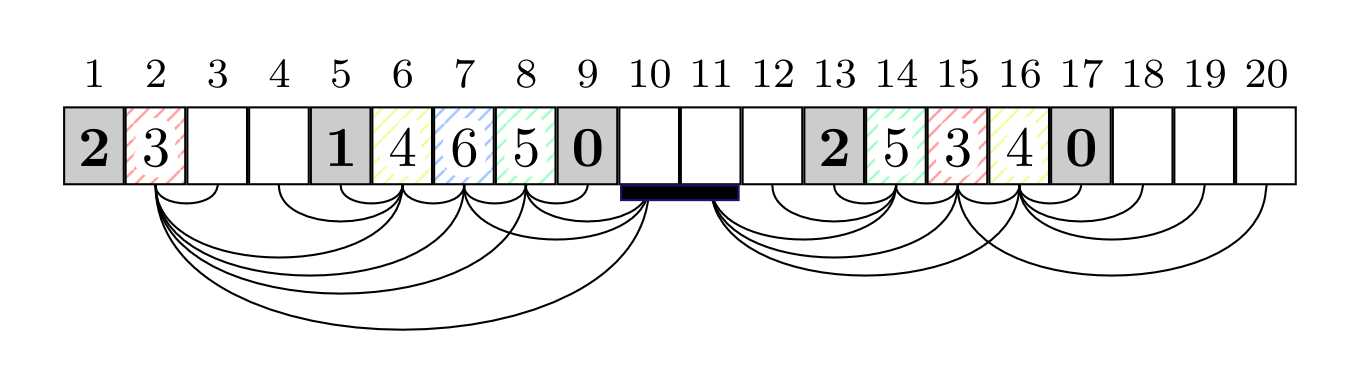
\includegraphics[width=0.5\textwidth]{pictures/squares_conflict.png}
    \end{center}

    Analysis of the conflict graph after the player terminates.
\end{frame}



%\begin{mylemblock}{\textbf{Lemma}}
%    \begin{tikzpicture}[overlay, remember picture]
%    \node (mark) {};
%    \end{tikzpicture}
%    {\small $\frac\strut\strut$A $\Delta$-approximate LZ factorisation can be computed in $\orderof{n + \frac{n \cdot \lg n \cdot \sigma}{\sqrt{\Delta}}}$ time.}
%\end{mylemblock}